% Do not delete this line (pandoc magic!)

\problem{65-I-2}{}{
Určte, koľkými spôsobmi možno k jednotlivým vrcholom kocky $ABCDEFGH$ pripísať čísla 1, 3, 3, 3, 4, 4, 4, 4 tak, aby súčin čísel pripísaných ľubovoľným trom vrcholom každej zo stien kocky bol párny.
}{
\rieh Pre kontrolu dotyčnej podmienky stačí vedieť len to, ktorým vrcholom kocky $ABCDEFGH$ sú pripísané čísla nepárne a ktorým čísla párne. Zaveďme preto znaky $N$ a $P$ pre všetky nepárne, resp. párne čísla a riešme najskôr otázku, koľkými vyhovujúcimi spôsobmi môžeme pripísať k vrcholom kocky $ABCDEFGH$ štyri $N$ a štyri $P$ (práve toľko ich totiž je medzi zadanými číslami 1, 3, 3, 3, 4, 4, 4, 4).

Uvedomme si, čo podmienka úlohy hovorí o počte znakov $N$ pripísaných vrcholom jednej a tej istej steny kocky: počet týchto $N$ je nanajvýš 2 (súčin troch pripísaných $N$ by bol totiž nepárny, teda v rozpore s danou podmienkou). Keď však danú stenu kocky zvážime súčasne so stenou s ňou rovnobežnou (t. j. stenou protiľahlou), pri ktorej vrcholoch sú tiež nanajvýš dve $N$, a zohľadníme pritom, že pri ôsmich vrcholoch týchto dvoch stien (teda pri všetkých ôsmich vrcholoch kocky) sú (všetky) štyri $N$, dôjdeme 1k záveru, že pri vrcholoch každej steny sú práve dve $N$ (a teda aj dve $P$). Naopak, každé také pripísanie štyroch $N$ a štyroch $P$ zrejme vyhovuje požiadavkám úlohy.

Stojíme tak pred úlohou určiť počet tých pripísaní štyroch $N$ a štyroch $P$ vrcholom kocky $ABCDEFGH$, pri ktorých sú dve $N$ a dve $P$ pri vrcholoch každej steny. Rozdelíme ich na dve skupiny podľa toho, či existuje stena, na ktorej sú obe $N$
priradené vrcholom susedným (na kocke tak vznikne aspoň jedna hrana ”$NN$“), alebo naopak vo všetkých stenách sú obe $N$ priradené vrcholom protiľahlým (všetky hrany kocky potom budú
”$N$P“). Po jednom reprezentantovi oboch skupín vidíme na obr. 1 -- pre lepší prehľad bez označenia vrcholov kocky písmenami. Ľahko overíme (výklad tu vynecháme), že znaky v krúžku pri reprezentantoch oboch skupín už jednoznačne určujú znaky pri všetkých ostatných vrcholoch kocky.
\begin{center}
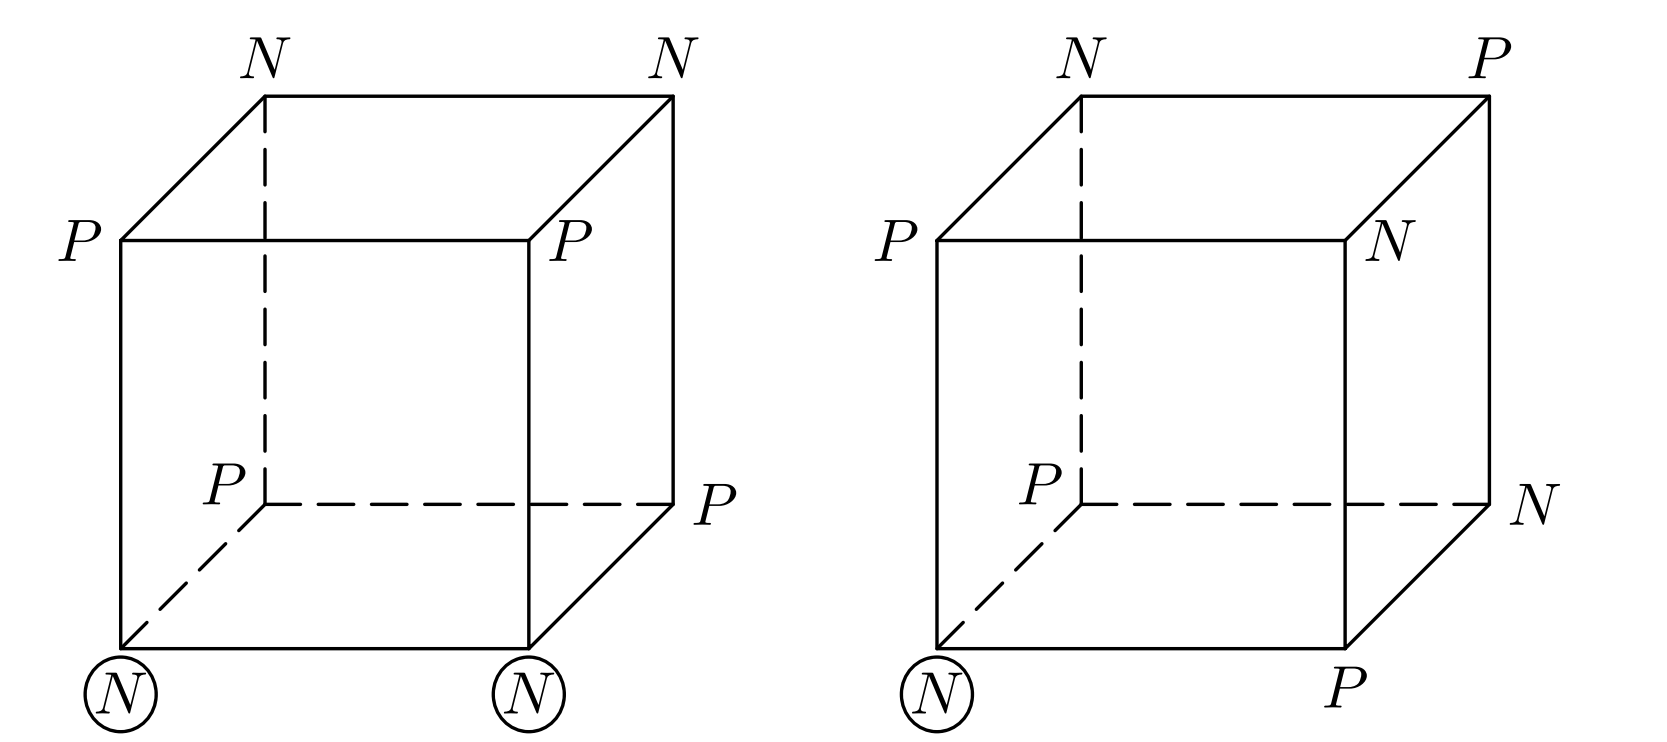
\includegraphics[width=0.6\textwidth]{NPkocka}
\end{center}

Teraz už ľahko usúdime, že v prvej skupine je práve šesť priradení -- jednou hranou ”$NN$“ je totiž, ako vieme, celé vyhovujúce priradenie určené a má práve dve hrany ”$NN$“, ktoré sú pritom rovnobežné a neležia v jednej stene; takých dvojíc hrán je pre kocku $ABCDEFGH$ práve šesť. Naproti tomu v druhej skupine sú iba dve rzne priradenia -- pretože sa jedná o priradenie bez hrany ”$NN$“; znakom $P$ alebo $N$ pri vrchole $A$ danej kocky sú totiž, ako vieme, určené znaky pri všetkých ďalších jej vrcholoch. Existuje tak spolu $6 + 2 = 8$ vyhovujúcich priradení štyroch $N$ a štyroch $P$ vrcholom kocky $ABCDEFGH$.

V ďalšej, jednoduchšej časti nášho postupu určíme, koľkými spôsobmi môžeme štyri $N$ a štyri $P$ (pevne pripísané vrcholom kocky) zameniť konkrétnymi číslami 1, 3, 3, 3, 4, 4, 4, 4. Máme zrejme práve štyri možnosti pre výber toho $N$, ktoré zameníme číslom 1; potom už zvyšné tri $N$ musíme zameniť číslom 3, rovnako ako všetky štyri $P$ číslom 4. Počet spôsobov zámen znakov $N$ a $P$ danými číslami je tak rovný 4.

Nakoniec uplatníme jednoduché kombinatorické pravidlo súčinu: keďže existuje osem vyhovujúcich pripísaní znakov $N$ a $P$ k vrcholom danej kocky a pri každom z nich možno štyrmi spôsobmi zameniť znaky $N$ a $P$ danými číslami, je hľadaný počet vyhovujúcich pripísaní daných čísel vrcholom danej kocky rovný $8 \cdot 4 = 32$.
}